\documentclass[12pt,oneside,a4paper,parskip]{scrbook}
\usepackage[utf8]{inputenc}
\usepackage[T1]{fontenc}
\usepackage{lmodern}
\usepackage{csquotes}
\usepackage[ngerman]{babel}
\usepackage{floatflt} 
\usepackage{subfigure}
\usepackage[pdftex]{graphicx}
\usepackage[hidelinks]{hyperref}
\usepackage{color}
\usepackage{amssymb}
\usepackage{textcomp}
\usepackage{nicefrac}
\usepackage{pdfpages}
\usepackage{float} 
\usepackage{pdflscape}
\usepackage{subfigure}
\usepackage{pdfpages}  
\usepackage[verbose]{placeins} 
\usepackage[nouppercase,headsepline,plainfootsepline]{scrpage2}
\usepackage{listings}		
\usepackage{xcolor}			
\usepackage{color}			
\usepackage{caption}		
\usepackage{subfigure}			
\usepackage{epstopdf}		
\usepackage{longtable}  
\usepackage{setspace}
\usepackage{booktabs}
\usepackage[style=numeric, backend=biber]{biblatex}
\bibliography{literatur2}
\usepackage[nolist]{acronym}
\usepackage{tikz}
\usetikzlibrary{arrows,automata}

%%%%%%%%%%%%%%%%%%%
%% definitions
%%%%%%%%%%%%%%%%%%%
\def\BaAuthor{Marcel Groß}
\def\BaTitle{Design und Implementierung eines Generators für Android View Komponenten}
\def\BaSupervisorOne{Prof.\ Dr.\ Peter Braun}
\def\BaSupervisorTwo{Prof.\ Dr.\ Steffen Heinzl}
\def\BaDeadline{31.03.2017}

\hypersetup{
pdfauthor={\BaAuthor},
pdftitle={\BaTitle},
pdfsubject={Subject},
pdfkeywords={Keywords}
}

%%%%%%%%%%%%%%%%%%%
%% configs to include
%%%%%%%%%%%%%%%%%%%
\colorlet{punct}{red!60!black}
\definecolor{background}{HTML}{EEEEEE}
\definecolor{delim}{RGB}{20,105,176}
\colorlet{numb}{magenta!60!black}

\definecolor{gray}{rgb}{0.4,0.4,0.4}
\definecolor{darkblue}{rgb}{0.0,0.0,0.6}
\definecolor{cyan}{rgb}{0.0,0.6,0.6}

\definecolor{pblue}{rgb}{0.13,0.13,1}
\definecolor{pgreen}{rgb}{0,0.5,0}
\definecolor{pred}{rgb}{0.9,0,0}
\definecolor{pgrey}{rgb}{0.46,0.45,0.48}

\lstset{
  basicstyle=\ttfamily,
  columns=fullflexible,
  showstringspaces=false,
  commentstyle=\color{gray}\upshape
  linewidth=\textwidth
}

\lstdefinelanguage{json}{
    basicstyle=\normalfont\ttfamily,
    numbers=left,
    numberstyle=\scriptsize,
    stepnumber=1,
    numbersep=8pt,
    showstringspaces=false,
    breaklines=true,
    backgroundcolor=\color{background},
    literate=
     *{0}{{{\color{numb}0}}}{1}
      {1}{{{\color{numb}1}}}{1}
      {2}{{{\color{numb}2}}}{1}
      {3}{{{\color{numb}3}}}{1}
      {4}{{{\color{numb}4}}}{1}
      {5}{{{\color{numb}5}}}{1}
      {6}{{{\color{numb}6}}}{1}
      {7}{{{\color{numb}7}}}{1}
      {8}{{{\color{numb}8}}}{1}
      {9}{{{\color{numb}9}}}{1}
      {:}{{{\color{punct}{:}}}}{1}
      {,}{{{\color{punct}{,}}}}{1}
      {\{}{{{\color{delim}{\{}}}}{1}
      {\}}{{{\color{delim}{\}}}}}{1}
      {[}{{{\color{delim}{[}}}}{1}
      {]}{{{\color{delim}{]}}}}{1},
}

\lstset{language=xml,
  morestring=[b]",
  morestring=[s]{>}{<},
  morecomment=[s]{<?}{?>},
  stringstyle=\color{black},
  numbers=left,
  numberstyle=\scriptsize,
  stepnumber=1,
  numbersep=8pt,
  identifierstyle=\color{darkblue},
  keywordstyle=\color{cyan},
  backgroundcolor=\color{background},
  morekeywords={xmlns,version,type}% list your attributes here
}

\lstset{language=Java,
  showspaces=false,
  showtabs=false,
  tabsize=4,
  breaklines=true,
  keepspaces=true,      
  numbers=left,
  numberstyle=\scriptsize,
  stepnumber=1,
  numbersep=8pt,
  showstringspaces=false,
  breakatwhitespace=true,
  commentstyle=\color{pgreen},
  keywordstyle=\color{pblue},
  stringstyle=\color{pred},
  basicstyle=\ttfamily,
  backgroundcolor=\color{background},
%  moredelim=[il][\textcolor{pgrey}]{$$},
%  moredelim=[is][\textcolor{pgrey}]{\%\%}{\%\%}
}

\begin{document}

\begin{acronym}[Bash]
	\acro{gemara}[GeMARA]{GEnerierung von Mobilen Applikationen basierend auf REST Architekturen}
	\acro{rest}[REST]{REpresentational State Transfer}
	\acro{ui}[UI]{User Interface}
	\acro{dsl}[DSL]{domänenspezifische Sprache}
\end{acronym}
%%%%%%%%%%%%%%%%%%%
%% Titelseite
%%%%%%%%%%%%%%%%%%%


\frontmatter
\titlehead{%  {\centering Seitenkopf}
  {Hochschule für angewandte Wissenschaften Würzburg-Schweinfurt\\
   Fakultät Informatik und Wirtschaftsinformatik}}
\subject{Bachelorarbeit}
\title{\BaTitle\\[15mm]}
\subtitle{\normalsize{vorgelegt an der Hochschule f\"{u}r angewandte Wissenschaften W\"{u}rzburg-Schweinfurt in der Fakult\"{a}t Informatik und Wirtschaftsinformatik zum Abschluss eines Studiums im Studiengang Informatik}}
\author{\BaAuthor}
\date{\normalsize{Eingereicht am: \BaDeadline}}
\publishers{
  \normalsize{Erstpr\"{u}fer: \BaSupervisorOne}\\
  \normalsize{Zweitpr\"{u}fer: \BaSupervisorTwo}\\
}

%\uppertitleback{ }
%\lowertitleback{ }

\maketitle


%%%%%%%%%%%%%%%%%%%
%% abstract
%%%%%%%%%%%%%%%%%%%

\section*{Zusammenfassung}

TODO

\section*{Abstract}

TODO

\newpage
\chapter*{Danksagung}



%%%%%%%%%%%%%%%%%%%
%% Inhaltsverzeichnis
%%%%%%%%%%%%%%%%%%%
\tableofcontents										



%%%%%%%%%%%%%%%%%%%
%% Main part of the thesis
%%%%%%%%%%%%%%%%%%%
\mainmatter

\chapter{Einführung}\label{ch:intro}

Das Smartphone ist heutzutage der stete Begleiter eines Menschen. \enquote{Zwei Drittel der Bevölkerung und nahezu jeder 14- bis 29-Jährige geht darüber ins Netz.} \cite{usage} Auch die Prognose zeigt, das der Absatzmarkt immer weiter steigen wird (Abbildung \ref{fig:prognose_fig}).

\begin{figure}[H]
	\begin{center}
		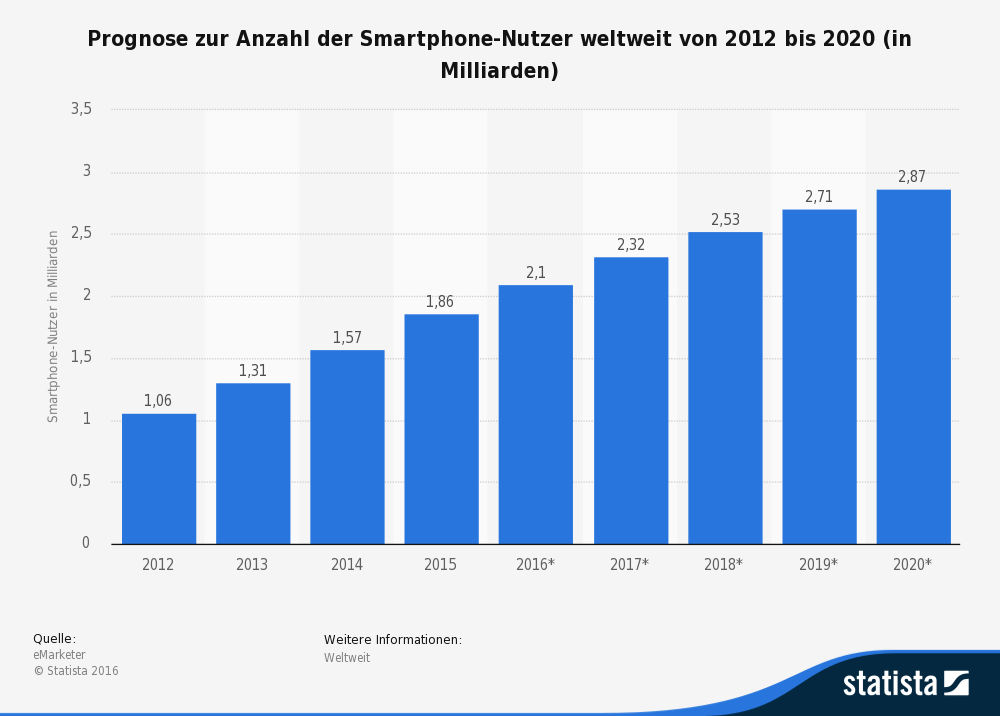
\includegraphics[width=0.86\textwidth]{images/prognose-zur-anzahl-der-smartphone-nutzer-weltweit-bis-2020.png}
		\caption{Prognose zur Anzahl der Smartphone-Nutzer weltweit von 2012 bis 2020 (in Milliarden) \cite{prognose}.}
		\label{fig:prognose_fig}
	\end{center}
\end{figure}

Umso wichtiger ist es, dass die Softwareentwicklung diesen Trend ernst nimmt. Der ehemalige Google-Chef Eric Schmidt sagte bereits 2010: \enquote{Googles Devise heißt jetzt \enquote{Mobile first}}. 
Diese Devise wird von vielen Unternehmen verfolgt und ist der Grund, weswegen in den einzelnen Stores gegenwärtig so viele Apps angeboten werden. Bei Android im Playstore waren im Oktober 2016 ca. 2,4 Millionen Apps \cite{play_store} und bei Apple im App Store ca. 2 Millionen Apps (Stand Juni 2016) verfügbar \cite{app_store}. Neben Googles Android und Apples iOS gibt es noch andere Betriebssysteme, wie beispielsweise Microsofts Windows Phone oder Blackberrys Blackberry OS. Jedoch dominieren die beiden erstgenannten Systeme derzeit den Markt (Abbildung \ref{fig:os_fig}).

\begin{figure}[H]
	\begin{center}
		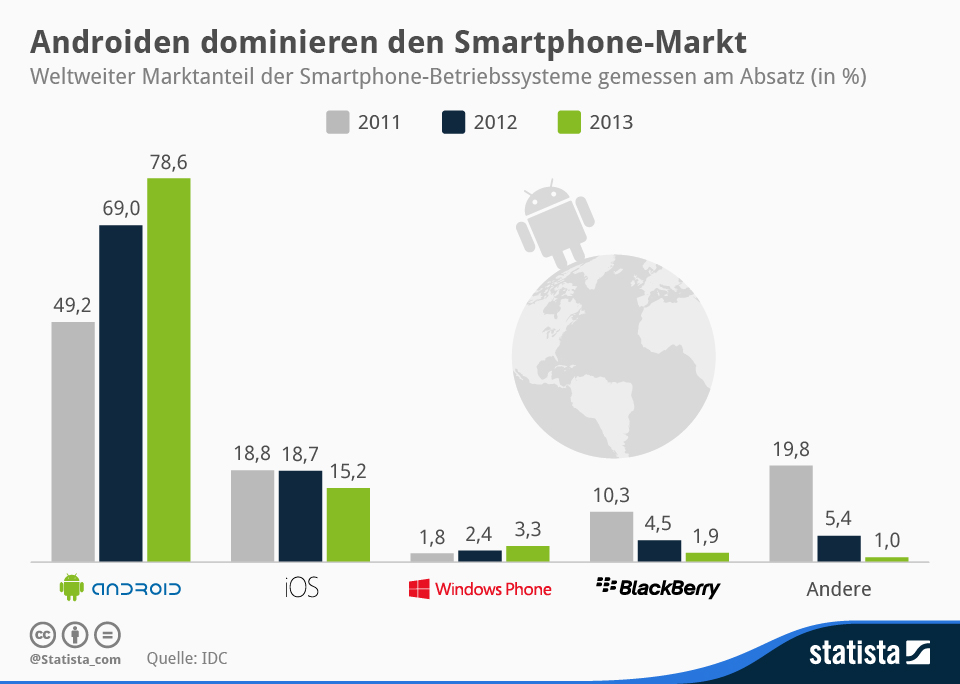
\includegraphics[width=0.86\textwidth]{images/os.jpg}
		\caption{Der weltweite Marktanteil an Smartphone-Betriebssystemen \cite{os}.}
		\label{fig:os_fig}
	\end{center}
\end{figure}

Jede dieser Applikationen wurde einzeln für sich entwickelt und implementiert. Bei jedem Update, zum Beispiel des Systems, müssen alle Anwendungen gewartet und überarbeitet werden, um die volle Funktionalität zu gewährleisten.

Würden einige Applikationen jedoch genauer analysiert werden, wäre das Ergebnis, dass Codepassagen in jeder dieser Anwendungen vorhanden sind, welche einen ähnlichen beziehungsweise denselben Zweck erfüllen. Werden diese Stellen im Programmcode abstrahiert, gibt es die Möglichkeit, diese generieren zu lassen, dafür werden so genannte Code-Generatoren benötigt. 

Im Bereich der Backend-Entwicklung gibt es bereits verschiedene Projekte die sich damit befassen. Ein Beispiel wäre der \textit{CRUD Admin Generator} \cite{generators}. Die Hochschule für angewandte Wissenschaften Würzburg-Schweinfurt entwickelt  unter der Leitung von Prof. Dr. Peter Braun auch einen Code-Generator unter dem Namen \ac{gemara}. Mit Hilfe solcher Generatoren für den Bereich Mobiler Applikationen könnte der Entwicklungs- und Wartungsaufwand reduziert werden. 

Führt ein Systemupdate dazu, dass die Implementierung verschiedener Anforderungen nicht länger funktionsfähig ist, muss dies nur einmalig an der entsprechenden Stelle im Code-Generator geändert werden und nicht in jeder Applikation einzeln. 

\section{Motivation}\label{sec:motivation}
Im Rahmen des Projektes \ac{gemara} gab es bereits Arbeiten, welche sich mit dem Thema der Generierung von \textit{Android Activities} beschäftigt. Die dabei entstandenen Lösungen resultieren darin, dass das Generieren von \textit{Activities} zu Problemen führt. Deshalb behandelt diese Ausarbeitung das Erzeugen von sogenannten Komponenten und nicht kompletter \textit{Activity}.

Eine Komponente ist im Wesentlichen eine kleine Anwendung für sich, welche nur eine einzige Aufgabe erfüllt. Dies könnte zum Beispiel das Anzeigen eines Dozenten in einer Campus-Applikation sein.
Aus den erzeugten Komponenten kann eine Art Bausatz entstehen, mit dessen Hilfe der Entwickler seine Applikation zusammen bauen kann. Dabei wird ihm freie Wahl gelassen, wie der Aufbau seiner Anwendung aussieht. Er bedient sich nur an gegebener Stelle an den Komponenten. Dadurch reduziert sich der Entwicklungsaufwand für ihn.

Bewegen wir uns in der Domain einer Hochschule, kann eine Bibliothek mit den erzeugten Komponenten allen Studierenden zur Verfügung gestellt werden. Dadurch wäre jeder Studierende in der Lage eine persönliche Campus-Applikation zu entwickeln. Durch die einzelnen Komponenten kann dann sichergestellt werden, dass grundsätzliche Funktionalität bereits gewährleistet ist.

\section{Zielsetzung}\label{sec:target}
Ziel dieser Ausarbeitung ist es, dass der Leser einen grundsätzlichen Überblick für die Entwicklung von Android Applikationen beziehungsweise Android-Bibliotheken vermittelt bekommt. Weiterhin soll das Wissen des Lesers über Datenkommunikation mittels \textit{\acf{rest}} vertieft werden. Hierbei wird der Schwerpunkt auf das \textit{Hypermedia-Prinzip} gelegt. 

Neben diesen spezifischen Anforderungen soll ein Verständnis der Implementierung von Generatoren entstehen. Dafür muss der Entwickler entscheiden können, was von der Implementierung als statischer Code angesehen werden kann und welcher generisch ist. Dieses Verständnis ist wichtig, um die Komplexität der Generatoren zu reduzieren. Da die statischen Anteile jedes Mal identisch sind.
Auch soll auf die Frage eingegangen werden, ob das \textit{\ac{ui}}, welches ebenfalls generiert wird, auch generisch gestaltet werden kann. Das bedeutet, dass nicht nur Informationen, welche angezeigt werden sollen, beschrieben werden, sondern auch, wie diese angezeigt werden sollen.

Wenn es möglich ist, dass das \textit{\ac{ui}} als Teil der \textit{domänenspezifischen Sprache (DSL)} beschrieben werden kann, so hat der Nutzer des entsprechenden Generators die Freiheit, selbst zu entscheiden, ob zum Beispiel in seiner Campus-App bei der Liste aller Dozenten das Profilbild links oder rechts angezeigt werden soll.

\section{Aufbau der Arbeit}\label{sec:structure}
Diese Ausarbeitung ist in sieben Kapitel unterteilt. In der Einführung wird zu Beginn auf den Stellenwert von Android Applikationen eingegangen. Im Kapitel Motivation wird die Problemstellung angerissen und zur Zielsetzung hingeführt. Mit dem Aufbau der Arbeit wird das Kapitel abgeschlossen.

Das zweite Kapitel befasst sich mit den Grundlagen. Hier soll der Leser noch einmal seinen Kenntnisstand über \textit{\acf{rest}} auffrischen und die Bedeutung von \textit{\acf{hateoas}} verstehen können. Neben dem Bereich der Netzwerkkommunikation wird außerdem noch der Bereich Android angeschnitten. Hier liegt der Schwerpunkt in der Entwicklung von Applikationen und \textit{CustomViews}. Dabei werden die einzelnen Schritte aufgezeigt, um diese Komponenten zu erstellen und zu benutzen. Der letzte Teil in den Grundlagen befasst sich mit Software-Generatoren. Der Leser erhält einen Einblick drüber, was eine \textit{\acf{dsl}} ist und in welche zwei generelle Arten diese eingeteilt werden. Im Anschluss folgt die Vorstellung des Projekts \acf{gemara}. 

Das dritte Kapitel behandelt die Problemstellung. Dabei wird die Referenzanwendung vorgestellt. Diese Vorstellung inkludiert sowohl das Backend als auch die Android Applikation. Es enthält weitergehend die Generierung des Backends mit Hilfe von \ac{gemara} und das Aussehen des daraus resultierenden \ac{api}. 
Anschließend wird die Android Anwendung analysiert. Dabei wird sowohl der Aufbau der Applikation als auch die einzelnen \textit{Views} betrachtet. Die Analyse des Aufbaus soll eine Einteilung in einen generischen sowie spezifischen Quellcode ermöglichen. Bei der Betrachtung der \textit{Views} sollen Gemeinsamkeiten im Aufbau und Design offenbart werden, so dass diese mit einer \textit{\ac{dsl}} modellierbar sind. Zum Abschluss wird das \textit{Meta-Modell} vorgestellt. Es wird auf die Anforderungen an dieses eingegangen und anschließend zwei weitere Modelle vorgestellt. Ein reines Android Modell und die Erweiterung des vorhandenen Enfield-Modells. Das \textit{Meta-Modell} wird dahingehend untersucht, um herauszufinden, welche Daten das \textit{Meta-Modell} benötigt. Bei dem analysieren der einzelnen \textit{Views} wird ein Augenmerk auf den Programmablauf und die Aktionen bei Klick gelegt. Anschließend folgt die Vorstellung des Aufbaus der \textit{View-Meta-Modelle}. Bei jeder \textit{View} wird auf deren Besonderheiten und Möglichkeiten eingegangen. Neben den \textit{View-spezifischen} Daten wird auch noch aufgezeigt, welche Dateien allgemein benötigt werden und wo deren Platzierung im vorgegebenen Modell ist.

Im Kapitel Lösung wird der in dieser Arbeit entwickelte Software-Generator \textit{Welling} vorgestellt.
Zunächst erfolgt die Vorstellung des \textit{Java \acf{api} JavaPoet} zur Generierung von Java-Klassen. Anschießend wird beschrieben, wie andere Datei-Typen generiert werden können. Es wird gezeigt, welche Features unterstützt werden müssen. Nachfolgend wird der Aufbau des Generators vorgestellt. Es wird auf die einzelnen Bereiche eingegangen und deren Aufgabe sowie Funktionsweise erklärt. Abgeschlossen wird das Kapitel mit einer Anleitung, wie die generierte Applikation gebaut und ausgeführt werden kann.

Das fünfte Kapitel, Evaluierung anhand einer Beispielanwendung, ist in drei Bereiche eingeteilt. Zunächst wird die Beispielanwendung vorgestellt. Anschließend wird auf die Erstellung und Nutzung des \textit{Meta-Modells} eingegangen, wobei hier auch Einschränkungen durch dieses aufgezeigt werden. Der letzte Bereich befasst sich mit dem Zeitaufwand und der Komplexität der Entwicklung, Wartung sowie Nutzung des Generators. Auch wird die Komplexität der erzeugten Applikation kritisch bewertet.

Im letzten Kapitel, Zusammenfassung, wird die Arbeit reflektiert und zusätzliche Erweiterungen und Ergänzungen an \textit{Meta-Modell} und Software-Generator dargestellt.

\chapter{Grundlagen}\label{ch:basics}
\section{\acf{rest}}\label{sec:rest}



\begin{figure}[H]
	\begin{center}
		\begin{tikzpicture}[->,>=stealth',shorten >=1pt,auto,node distance=3cm,
		semithick]
		\tikzstyle{every state}=[fill=none,text=black]
		
		\node[initial,state] (A) [minimum width=3cm]             {Dispatcher};
		\node[state]         (B) [right of=A, minimum width=2cm] {Collection};
		\node[state]         (D) [below of=B, minimum width=2cm] {Create};
		\node[state]         (C) [right of=B, minimum width=2cm] {Single};
		\node[state]         (E) [above of=C, minimum width=2cm] {Delete};
		\node[state]		 (F) [below of=C, minimum width=2cm] {Update};
		
		\path 
		(A) edge             (B)
		(B) edge [bend left] (C)
			edge [bend left] (D)
		(C)	edge 			 (E)
			edge [bend left] (B)
			edge [bend left] (F)
		(D) edge [bend left] (B)
		(E) edge   			 (B)
		(F) edge [bend left] (C);
		
		\end{tikzpicture}
	\end{center}
\end{figure}

\section{Android}\label{sec:android}
\subsection{Custom Views}
Noch mehr Text


\section{Generatoren}\label{sec:generators}
\subsection{\acf{gemara}}\label{sec:gemara}

\chapter{Problemstellung} \label{ch:problem}
\section{Meta-Model und Android Applikation spezifisches}
Bei der Generierung von Android Applikations gibt es vieles zu berücksichtigen. Angefangen bei den einfachsten Möglichkeiten zur Darstellung von Schrift. In welcher Farbe oder Größe sollte sie dargestellt werden. 

Wie soll eine View an sich aufgebaut sein? Wie sind die zu repräsentierenden Daten aufbereitet?
Soll der Vorname eine Zeile über dem Nachnamen stehen? Oder soll es genau umgekehrt sein? Es gibt auch noch die Möglichkeit der Kombination. Vorname und Nachname in einer Zeile, oder Nachname und Vorname in einer Zeile. 

Was soll überhaupt dargestellt werden? Gehen wir vom Beispiel Person aus, soll nur der komplette Name dargestellt werden oder nur ein Teil des Namens. Was ist mit dem Geburtstag oder dem Wohnort. Gibt es zu der Person ein Profilbild? Was passiert wenn nicht alle Personen ein Profilbild haben, aber es soll ein Profilbild angezeigt werden? 
Das sind ein Teil der Fragen, die sich rein auf das \acf{ui} beziehen. Es gibt aber noch weiter Fragen die gestellt werden müssen. Soll es die Möglichkeit geben, das Aktionen beim Klick auf die Telefonnummer, E-Mail oder Homepage einer Person klickt ausgefüht werden?

Oder noch elementarer, welche Ansichten soll es überhaupt geben? Listen von Personen, Detailansichten und so weiter. 
Soll es die Möglichkeit geben neue Personen anzulegen, wenn ja was sind Pflichtangaben zu einer Person?
Dürfen bestehende Personen bearbeiten werden können?

Die letzten Fragen bezogen sich auf mögliche Funktionalitäten der Anwendung. Im letzten Bereich, gibt es noch Fragen, bezüglich des Ablaufes in einer Applikation. Welche View kommt nach welcher Aktion, wie sieht der Flow innerhalb einer Applikation aus.

Die oben genannten Fragen sind nur Beispiele für Überlegungen welche betrieben werden müssen um eine Android Anwendung zu entwickeln, das unterscheidet sich nicht vom normalen Entwicklungsprozess einer Anwendung.
Die große Frage hinter den aufgezählten Problemstellungen ist, wie können diese Anforderungen soweit abstrahiert werden, das diese Möglichst einfach mit einer \acf{dsl} beschrieben werden können.

Wurde ein geeignetes Meta-Model gefunden, so bleibt noch der Aspekt, dass der Software-Generator als Modul von \acf{gemara} entwickelt werden soll. \acs{gemara} bringt ein bereits bestehende Meta-Model und wiederum eigene Anforderungen mit sich. Durch den auf \acf{rest}, basierenden Architekturstil bringt es beispielsweise die Anforderung mit, dass eine Anwendung mit Hilfe eines endlichen Automaten designed werden soll. Das bedeutet, dass die States und Transitionen des endlichen Automaten den Ablauf in der Applikaition vorgeben.
Es wäre auserdem noch wünschenswert, dass die Erweiterung des Meta-Models nicht ausschließlich für Android Applikationen, sondern für jegliche Client Anwendungen genutzt werden kann.

Aus den oben erörterten Fragen und Problemstellungen, welche nur beispielhaft und nicht komplett sind, lassen sich nun folgende Kategorien ableiten.

\begin{itemize}
	\item Beschreibung des \acl{ui}.
	\item Beschreibung der Aktionen bei Klick.
	\item Beschreibung der Architektur und des Ablaufs innerhalb der Applikation.
	\item Kompatiplität mit \acs{gemara} und andern möglichen Clients. 
\end{itemize}

Diese müssen für das Design und die Entwicklung eines Software-Generators für Android Applikationen beachtung finden.

\section{Design des Software-Generators}

Dieses Kaptiel zeigt Probleme und Fragenstellungen rund um den Generator an sich auf. Selbst wenn ein ein geeignetes Meta-Model besteht, heißt dass noch nicht, dass es auch einen funktionierenden Software-Generator gibt. Es gibt noch zu viele offene Punkte, wobei der Einfachste lautet: Muss alles generiert werden, oder gibt es Dateinen, welche kopiert werden können? Macht es Sinn, die Andorid Anwendung vorher soweit zu abstrahieren, das es möglichst wenig spezifischen Code und viel generischen Code gibt? Wie wird der Generator gesteuert, können die Dateien einfach so generiert werden, oder gibt es Abhängigkeiten untereinander? Was gibt es beim generieren von Klassen zu beachten? Beispielsweise müssen Activies in der \enquote{AndroidManifest.xml} registiert werden oder Strings sollten in einer \enquote{strings.xml} stehen und im Programmcode sollte nur mit Ids darauf referenziert werden.

Der Ablauf, wie wann was generiert wird muss teilweise im Meta-Model und teilweise im Generator selbst festgelegt werden. Da stellt sich wieder die Frage, was wird wo geregelt? 

Für Android Applikationen werden die verschiedensten Arten von Dateien benötigt. Angefangen mit Java-Klassen und XML-Dateien über Gradle-Dateien und \acfp{jar}.
Das wiederum wirft die Frage auf wie können die einzelnen Datei-Typen generiert und oder kopiert werden?


\chapter{Lösung}
In diesem Kapitel wird der in dieser Arbeit entwickelte Software-Generator \textit{Welling} vorgestellt. \textit{Welling} nutzt das zuvor beschriebene \textit{Meta-Modell}, um Android Applikationen generieren zu lassen. 

\section{Design des Software-Generators}
In diesem Kapitel soll auf die Problematik einen Software-Generator zu designen eingegangen werden. Ein funktionsfähiger Software-Generator benötigt neben einem geeigneten \textit{Meta-Modell} einen sinnvollen Aufbau. Der Aufbau bestimmt im Zusammenspiel mit dem \textit{Meta-Modell}, an welcher Stelle im zeitlichen Verlauf welche Klassen der Android Applikation generiert werden. Das ist wichtig, da für eine Anwendung die ausschließlich eine Liste darstellen beispielsweise keine Klassen für die Neuanlage von Datensätzen generiert werden sollen. 
Auch gibt es in Android Applikationen Abhängigkeiten zwischen verschiedenen Klassen. So müssen beispielsweise alle genutzten \textit{Activities} in der sogenannten \textit{AndroidMainfest.xml} registriert werden. Alle verwendeten Strings sollten nicht im Programmcode stehen, sondern ausgelagert in einer \textit{strings.xml} zu finden sein. Im Programmcode werden diese Strings dann mit Identifikatoren referenziert. Der Generator muss in der Lage sein, diese Abhängigkeiten in der Applikation darzustellen. 

Eine Android Applikation besteht neben Java- und XML-Klassen zusätzlich noch aus \textit{Gradle}-Dateien und \textit{\acfp{jar}}. Es ist nicht sinnvoll alle Dateien zu generieren. Bei manchen der Dateien ist es besser, diese an die entsprechende Stelle zu kopieren.

\subsection{Generierung der Java Klassen mit \textit{JavaPoet}}
\textit{JavaPoet} ist ein Java \textit{\ac{api}}, welches ermöglicht Java-Klassen zu generieren \cite{poet}. Hierfür wird die zu generierende Klasse programmiert. Mit Hilfe von nur ein paar Schlüsselwörtern ist es möglich, \textit{Klassen}, \textit{Interfaces} oder \textit{Methoden} zu generieren. 

Da der größte Teil des Generators Java-Klassen erzeugen muss, ist dieses \ac{api} bestens für diesen Zweck geeignet. Sie erspart die aufwändige String-Manipulation. Durch die Nutzung wird auch bei der Ausführung des Programms sichergestellt, dass gültige Konventionen und Regeln von Java eingehalten werden. So ist der grundsätzlich korrekte Aufbau einer Java-Klasse bereits vorab sichergestellt.

Listing \ref{lst:poet} zeigt ein einfaches Beispiel zur Generierung einer Hello-World-Klasse und Listing \ref{lst:poet_result} zeigt das Ergebnis nach der Ausführung des Beispiels. Der korrekte Aufbau eine Java Klasse wurde durch JavaPoet erzeugt. Dabei wurden die Konventionen wie \textit{camel-case} eingehalten.

\begin{lstlisting}[label=lst:poet,
language=java,
firstnumber=1,
caption=Beispiel für die Generation einer Hallo-World-Klasse mit JavaPoet \cite{poet}.]				   
MethodSpec main = MethodSpec.methodBuilder("main")
	.addModifiers(Modifier.PUBLIC, Modifier.STATIC)
	.returns(void.class)
	.addParameter(String[].class, "args")
	.addStatement("$T.out.println($S)", System.class, "Hello, JavaPoet!")
	.build();

TypeSpec helloWorld = TypeSpec.classBuilder("HelloWorld")
	.addModifiers(Modifier.PUBLIC, Modifier.FINAL)
	.addMethod(main)
	.build();

JavaFile javaFile = JavaFile.builder("com.example.helloworld", helloWorld)
	.build();
\end{lstlisting}

\begin{lstlisting}[label=lst:poet_result,
language=java,
firstnumber=1,
caption=Ergebnis der Generation von Listing \ref{lst:poet} \cite{poet}.]				   
package com.example.helloworld;

public final class HelloWorld {
	public static void main(String[] args) {
		System.out.println("Hello, JavaPoet!");
	}
}
\end{lstlisting}

\newpage

\subsection{Generierung anderer Datentypen}

Neben Java-Klassen besitzt der Quellcode einer Android Applikation auch \textit{XML}-Dateien und \textit{Gradle}-Dateien. Für diese Typen muss eine andere Möglichkeit der Generierung gewählt werden. Hierfür liefert die \acf{gemara} mit der Klasse \textit{GeneratedFile} eine Möglichkeit. Diese Klasse besitzt die beiden Methoden \textit{append(String content)} und \textit{appendln(String content)}, welche ermöglichen, jedes beliebige textbasierte File-Format zu generieren. Ein \textit{GeneratedFile} Objekt erzeugt eine Datei, durch welche mit den beiden erwähnten Methoden Strings hinzugefügt werden können. Dadurch wird die Möglichkeit eröffnet, jede beliebige Textstruktur zu erzeugen. Jedoch liefert diese Klasse keinerlei Validierung. Die Datei wird generiert, egal ob die Struktur gültig ist oder nicht.

Listing \ref{lst:append} erzeugt eine in Listing \ref{lst:append_result} dargestellte Datei \textit{test.xml} unter dem Verzeichnis \textit{generated}.
\begin{lstlisting}[label=lst:append,
language=java,
firstnumber=1,
caption=Beispiel eine \textit{GeneratedFile}-Instanz zur Erzeugung einer \textit{XML}-Datei.]				   
public class FileGenerator extends GeneratedFile {

	@Override
	public void generate() {
		appendln("<?xml version=\"1.0\" encoding=\"utf-8\"?>");
		appendln("<menu xmlns:android=\"http://schemas.android.com/apk/res/android\" xmlns:app=\"http://schemas.android.com/apk/res-auto\">");
		appendln("<item android:id=\"@+id/saveItem\"");
		appendln("android:title=\"@string/save\"");
		appendln("app:showAsAction=\"always\"\\>");
		appendln("<\\menu>");
	}

	@Override
	protected String getFileName() {
		return "test.xml";
	}

	@Override
	protected String getDirectoryName() {
		return "/generated";
	}
}
\end{lstlisting}

\newpage

\begin{lstlisting}[label=lst:append_result,
language=xml,
firstnumber=1,
caption=Erzeugte \textit{XML}-Datei durch den Quellcode von Listing \ref{lst:append}.]				   
<?xml version="1.0" encoding="utf-8"?>
	<menu xmlns:android="http://schemas.android.com/apk/res/android"
		xmlns:app="http://schemas.android.com/apk/res-auto">
		<item android:id="@+id/saveItem"
			android:title="@string/save"
			android:icon="@drawable/ic_done"
			app:showAsAction="always"/>
	</menu>
\end{lstlisting}

\subsection{Ablauf der Generierung}
Um eine Android Applikation generieren zu lassen, müssen nicht alle Klassen ein Generat sein. Es können auch Überlegungen angestrebt werden, generische Klassen einfach im Generator abzulegen und bei Bedarf zu kopieren. Diese Methode wurde verworfen, da andernfalls jedes Mal die kopierten Klassen via String-Manipulation bearbeitet werden müssten. Die minimale Änderung, welche immer wieder getroffen werden müsste, wäre das Anpassen der \textit{Package} Anweisung am Anfang der Java-Klassen und die der \textit{Import}-Anweisungen. Eine weitere Überlegung wäre, diese Klassen in eine Android Bibliothek auszulagern, und dann in jede Anwendung zu importieren. Auch von dieser Möglichkeit wurde in der ersten Version abgesehen, da die Applikation bereits aus zwei Komponenten besteht: der Applikation an sich und einer Bibliothek, welche die Android-Komponenten für die Anwendung enthält. Um die Komplexität zu reduzieren, werden die benötigten generischen Klassen als Teil der eingebunden Bibliothek fortwährend aufs Neue generiert.

\subsection{Aufbau des Generators}

\begin{figure}[H]
	\begin{center}
		\includegraphics[width=\textwidth]{images/Welling.png}
		\caption{Aufbau des Android-Generators Welling.}
		\label{fig:welling}
	\end{center}
\end{figure}


Die Klasse \textit{ApplicationGenerator} ist der Einstiegspunkt des Projekts. Sie erwartet im Konstruktor ein \textit{Enfield-Modell} Objekt. Wie der Abbildung \ref{fig:welling} entnommen werden kann, lässt sich das Projekt in drei Teilbereiche gliedern. Der erste Bereich erzeugt ein \textit{AppDescription} Objekt (Abbildung \ref{fig:appDescription}), der zweite Bereich befasst sich mit allgemeinen Vorbereitungen, die getroffen werden müssen und der letzte iteriert über die \textit{States}, und generiert nach Bedarf die benötigten Klassen.

Die \textit{ApplicationGenerator} Klasse verfügt über eine öffentliche Methode \textit{generate}. Beim Aufrufen dieser Methode werden die einzelnen Generatoren für den allgemeinen Bereich angestoßen. Weiterhin wird das Iterieren über die \textit{States} des \textit{Enfield-Modell} begonnen. Zum Schluss wird noch das \textit{AppDescription} Objekt ausgewertet, die darin enthaltenen Informationen in Dateien geschrieben und an der entsprechenden Stelle im Projekt gespeichert.

\subsubsection{Erstellung der \textit{AppDescription}}

\begin{figure}[H]
	\begin{center}
		\includegraphics[width=\textwidth]{images/AppDescription.png}
		\caption{Aufbau des \textit{AppDescription} Objekts.}
		\label{fig:appDescription}
	\end{center}
\end{figure}

In der \textit{AppDescription} werden alle allgemeinen Daten durch den Generator gereicht, welche an mehreren Stellen benötigt werden, zum Beispiel der Name der Anwendung oder der Bibliothek. In jeder Java-Klasse muss der Paketname vorgehalten werden. Da sich diese in der Bibliothek und in der normalen Applikation unterscheiden, müssen diese für beide mitgeführt werden. Auch muss der Generator wissen, unter welchen Verzeichnissen die aktuelle Datei egal ob Java Klasse oder \textit{XML}-Datei, gespeichert werden soll. 
Diese Informationen können einfach aus dem \textit{Enfield-Modell} abgelesen werden. Auch die Ressourcen und die jeweiligen Subressourcen können direkt aus dem \textit{Meta-Modell} entnommen werden.  Dies ist der Teil des Initialisierens der \textit{AppDescription}. Alle bereits verfügbaren Informationen werden der \textit{AppDescription} zugewiesen. 

\newpage

Neben diesen Daten, die an mehreren Stellen bei der Generierung benötigt werden, gibt es Dateien in einer Android-Applikation, die sich während des Generierens aufbauen. Ein Beispiel für eine solche Datei ist die \textit{strings.xml}. 
Es wird in dem generierten Projekt zwei hiervon geben: eine im Bereich der Applikation selbst und eine weitere in der Bibliothek. Diese Dateien enthalten neben dem Applikationsnamen, beziehungsweise dem Bibliotheksnamen auch viele Strings, die beispielsweise erst in einem Fragment auftauchen. Jedoch müssen die benötigten Datensätze in die \textit{strings.xml} eingetragen werden. Um zu verhindern, dass der Generator die \textit{strings.xml} mehrfach erweitern muss, wird die \textit{AppDescription} in den entsprechenden \textit{AppString}-Attributen \textit{appString} beziehungsweise \textit{libString} erweitert.

Auch das \textit{AndroidManifest} wächst mit der Anwendung. So muss jede benutzte \textit{Aktivity} dort eingetragen sein, andernfalls kann diese nicht genutzt werden. Am Anfang des Generierens ist die genaue Anzahl und die Namen der \textit{Activities} unbekannt, weswegen der Generator diese beim Erzeugen zur \textit{AppDescription} hinzufügen muss. 
Das Attribut \textit{appDeclareStyleable} enthält alle \textit{CustomViews}, welche, wie im Kapitel \ref{sec:custom_view}, in die \textit{attr.xml} eingetragen werden müssen.

Da die Anwendung, welche generiert wird, auch den \acf{rest} Ansätzen entsprechen soll, muss diese wissen, welche \textit{Relationstypen} zu welchen Endpunkten gehören. Anfangs sind diese \textit{Relationstypen} ebenfalls unbekannt und werden erst im weiteren Verlauf beim Iterieren über die \textit{States} bekannt und zur \textit{AppDescription} hinzugefügt.
So wächst die \textit{AppDescription} über den gesamten Prozess des Generierens. Am Ende werden die gesammelten Daten in die entsprechenden Dateien an den jeweiligen Orten gespeichert. Das Verwenden und Weiterreichen eines \textit{AppDescription} Objekts reduziert die Komplexität des Generators. Der Generator muss deshalb nicht bei jeder Ergänzung einer der beschriebenen Dateien diese Aufrufen, den neuen Datensatz aufwändig hinzufügen und die Datei wieder abspeichern. Stattdessen muss der Generator die Datei nur einmal schreiben, da er zu Beginn des Schreibvorgangs alle von der Android Anwendung benötigten Informationen besitzt.

\subsubsection{Vorbereitung und Generierung allgemeiner Dateien}

Der Bereich zur Vorbereitung und Generierung der allgemeinen Dateien gliedert sich ebenfalls in drei Bereiche. Der erste Bereich behandelt alle Dateien, die von \textit{Gradle} benötigt werden. 

Er kopiert Daten, wie die \textit{gradlew.bat}, \textit{gradlew}, \textit{build.gradle} und den \textit{Gradle Wrapper}. 
Neben dem Kopieren werden sowohl für die Applikation und Bibliothek, als auch für das Gesamtprojekt die spezifischen Dateien generiert. So wird beispielsweise auf der Projektebene eine \textit{settings.gradle} oder in der Applikation sowie der Bibliothek jeweils eine \textit{build.gradle} erzeugt.

In der Sektion der Vorbereitung für die Applikation werden Dateien erzeugt, die jede Applikation benötigt, unabhängig von ihrem Aufbau oder deren Features. Es wird beispielsweise die \textit{MainActivity} oder die \textit{XML}-Dateien erzeugt, welche für die \textit{Transitions-Animationen} verantwortlich sind. Auch die \textit{styles.xml} wird generiert. Am Schluss werden noch die \textit{mipmap}-Ordner an die richtige Stelle kopiert.

Der Bereich, welcher die Bibliothek initialisiert, ist der Größte. Er generiert alle generell essentiellen Klassen. Darunter fallen die Klassen der Netzwerkkommunikation, die Klasse für das Link-Objekt sowie das Interface \textit{Resource}. Des Weiteren werden auch die größten Teile der in der Abbildung \ref{fig:lecturer_structure} abgebildeten generischen Klassen erzeugt. Auch die definitiv benötigten \textit{CustomViews} bereits generiert, inklusive deren \textit{XML}-Dateien. Für die Bibliothek kann beispielsweise das Manifest vorab erzeugt werden, da hier keine \textit{Activities} registriert werden müssen. Nach dem Ausführen des \textit{PrepareLibGenerators} steht das Grundgerüst der Bibliothek. Diese enthält alle bereits vorab erzeugbaren und benötigten Dateien, welche unabhängig von der gewünschten Funktion der Applikation benötigt werden. 

Der gesamte Teilbereich des Projekts befasst sich damit, ein Grundgerüst für die komplette Android Applikation zu erzeugen und vorab alle benötigten Dateien aufzubereiten. Die generierten Klassen haben jedoch noch keinerlei Programmlogik, die den spezifischen Ablauf der zu generierenden Anwendung steuert.

\subsubsection{Iterieren über die \textit{States}}

Der Teilbereich, der sich mit dem Iterieren über die einzelnen \textit{States} beschäftigt ist der komplexeste Bereich des Generators. Er ist dafür verantwortlich, dass zu jedem \textit{State} alle benötigten Klassen und Dateien generiert werden. 

Um diese Anforderung zu erfüllen, nutzt er den \textit{Visitor} \textit{IStateVisitor}, welcher durch das \textit{Enfield-Modell} zur Verfügung gestellt wird. Außerdem wird auch der \textit{Visitor} \textit{VisitStatesOnlyOnce} benutzt. Dieser zweite \textit{Visitor} stellt sicher, dass jeder \textit{State} nur einmal besucht wird. Würde der Generator einfach nur über die Transitionen der \textit{States} gehen, könnte es passieren, dass er in einer Endlosschleife endet. Gelangt der Generator zu einem \textit{State}, wird dieser mit dem \textit{IStateVisitor} identifiziert von welchem Typ dieser ist. Mögliche \textit{Statetypen} sind: ein \textit{State}, welcher einen \textit{GET-Request} auf eine einzelne Ressource oder auf eine Collection beschreibt oder \textit{States}, welche einen \textit{POST-}, \textit{PUT-} oder \textit{DELETE-Request} repräsentieren.  Nach dieser Identifikation wird bei jedem \textit{State}, außer dem \textit{DELETE-State}, eine Klasse für die in diesem \textit{State} betroffene Ressource erzeugt. Hierfür wird der \textit{ResourceGenerator} benutzt, auch wenn dabei die Ressource mehrfach angelegt werden würde. Der Generator überschreibt eine bereits angelegte Ressource. Diese Redundanz garantiert, dass auf jeden Fall eine Ressource zum betreffenden \textit{State} existiert. 

Neben diesen Ressource-Klassen wird auch ein \textit{StateHolder}-Objekt erstellt. Die Abbildung \ref{fig:stateHolder} repräsentiert dieses. 

\begin{figure}[H]
	\begin{center}
		\includegraphics[width=0.3\textwidth]{images/StateHolder.png}
		\caption{Aufbau des \textit{StateHolder} Objekts.}
		\label{fig:stateHolder}
	\end{center}
\end{figure}

Dieses Objekt wird für jeden einzelnen \textit{State} angelegt. Es enthält alle \textit{States}, welche über die \textit{Transitionen} erreicht werden können.
So weiß der Generator genau, ob beispielsweise ein \textit{Button} angezeigt werden muss, der eine Neuanlage einer Ressource ermöglicht. Diese Informationen stecken zwar auch im \textit{Enfield-Modell}, jedoch müsste jedes Mal, wenn überprüft werden soll, welche \textit{Folgestates} ein \textit{State} besitzt, über alle \textit{States} iteriert werden. Das \textit{StateHolder}-Objekt beschreibt sozusagen eine Landkarte für jeden einzelnen \textit{State}.

Der \textit{State}, welcher für das Löschen einer Ressource verantwortlich ist, ist der einfachste zu generieren. Hierfür wird lediglich ein \textit{DialogFragment} erzeugt, welches für das Löschen verwendet wird. 

Die anderen \textit{States} beinhalten mehr Klassen und Dateien. Außerdem werden die \textit{ResourceViews} (Kapitel \ref{sec:resourceViews}) benötigt, die jedem \textit{State} angehängt sind. Zur Identifizierung der einzelnen \textit{ResourceViews} wird wiederum mit dem \textit{Visitor-Pattern} gearbeitet. Die Klasse der \textit{ResourceView} stellt den \textit{Visitor} \textit{ResourceViewVisitor} zur Verfügung. 
Nachdem bekannt ist, welcher der drei \textit{ResourceView}-Typen im entsprechenden \textit{State} verwendet wurde, kann einer der Komponentengeneratoren - \textit{InputViewGenerator}, \textit{CardViewGenerator} oder \textit{DetailViewGenerator} - alle notwendigen Dateien generieren.

\begin{figure}[H]
	\begin{center}
		\includegraphics[width=\textwidth]{images/Lecturer-Swimlines.png}
		\caption{Aufbau der Dozenten Applikation mit Einteilung in spezifische \textit{States}.}
		\label{fig:swimlines}
	\end{center}
\end{figure}

In Abbildung \ref{fig:swimlines} ist die Applikation für Dozenten noch einmal abgebildet. Zur Vereinfachung wurde bei diesem Diagramm jedoch die Ressource Ämter mit ihren zugehörigen Klassen weggelassen.

Der Bereich \textit{Update} und der Bereich \textit{Create} werden hierbei vom \textit{InputViewGenerator}, der Bereich \textit{Read Collection} von \textit{CardViewGenerator} und der Bereich \textit{Read Single} vom \textit{DetailViewGenerator} erzeugt.
Jeder der einzelnen Generatoren ist ein Zusammenschluss von vielen Teilgeneratoren. Dabei werden in einem der Generatoren nicht nur die Java-Klassen für Applikation oder Bibliothek, sondern auch alle benötigten \textit{XML}-Dateien erzeugt.

\newpage

So ist beispielsweise der \textit{DetailViewGenerator} dafür verantwortlich, dass auf der Seite der Applikation, die \textit{LecturerDetailActivity} inklusive ihrer XML-Datei erzeugt wird. Er muss weitergehend auch diese \textit{Activity} in die \textit{AppDescription} im Bereich des \textit{Manifests} hinterlegen. Im Bereich der Bibliothek muss dafür gesorgt werden, dass die generischen Klassen \textit{ResourceDetailActivity} und \textit{ResourceDetailView} sowie die spezifischen Klassen \textit{LecturerDetailView}, \textit{LecturerDetailAdapter}, \textit{LecturerDetailViewHolder} und \textit{LecturerDetailCardView} erzeugt werden. Zu all diesen Klassen müssen mögliche Strings oder \textit{CustomViews} in die \textit{AppDescription} aufgenommen werden. Wiederum müssen auch die entsprechenden \textit{XML}-Dateien erzeugt werden. 

Jeder Generator besitzt mehrere Möglichkeiten, welche Klassen generiert werden müssen. Ob eine \textit{Activity} mit einer \textit{CollapsingToolbar} verwendet wird oder ob ein einfaches \textit{Fragment} zur Detailanzeige ausreichend ist, hängt davon ab, ob die Ressource ein Bild besitzt oder nicht.
Selbst die Generatoren auf der untersten Ebene, welche die einzelne Klassen erzeugen, wissen mit Hilfe von dem mitgegebenen \textit{StateHolder}, ob beispielsweise Menüeinträge für das Löschen oder das Bearbeiten von Ressourcen benötigt werden. Diese Generatoren richten sich auch nach den übergebenen \textit{RessourceViews}. Auf dieser Ebene haben die vom Benutzer des Generators mitgegebenen Informationen zum Aussehen Einfluss. Hier werden die benötigten Attribute der Ressource hinzugefügt und deren Aussehen in den entsprechenden \textit{XML}-Dateien beschrieben.


\section{Bauen und Ausführen der generierten Android Applikation}

Wurden alle benötigten Dateien der Applikation erzeugt, gibt es zwei Möglichkeiten, die Applikation zu bauen und anschließend auf einem Android-Endgerät zu installieren.

Variante 1: Importieren der generierten Dateien in eine Integrierte Entwicklungsumgebung (IDE), beispielsweise Android Studio. Dort, wie bereits bekannt, die Anwendung bauen und auf einem im Entwicklermodus befindlichen Android-Endgerät installieren.

Variante 2: Die Applikation mit Hilfe des \textit{Makefile} bauen und installieren. Hierfür muss ebenfalls ein Android-Endgerät im Entwicklermodus an den entsprechenden Computer angeschlossen sein.

\newpage

\begin{lstlisting}[label=lst:make,
language=xml,
firstnumber=1,
caption=\textit{Makefile} für das Bauen und Installieren der erzeugten Applikation.]				   
APK = gemara/android/src-gen/generated/app/build/outputs/apk/app-debug.apk

all: debug install

debug:
cd gemara/android/src-gen/generated && chmod 777 gradlew && ./gradlew clean assembleDebug

install:
adb $(TARGET) install -rk $(APK)
\end{lstlisting}

Listing \ref{lst:make} zeigt das \textit{Makefile}, welches die Möglichkeit bietet, entweder mit dem Befehl \textit{make} eine Debug-Version der Anwendung zu bauen und zu installieren oder mit dem Befehl \textit{make debug} ausschließlich die Applikation zu bauen, beziehungsweise mit dem Befehl \textit{make install} die bereits gebaute Applikation zu installieren.


\chapter{Evaluierung anhand einer Beispielanwendung}
Dieses Kapitel befasst sich mit dem Pro und Contra des Generierens einer Android Applikation, nach der in dieser Arbeit vorgestellten Methode.
Hierfür wird die Erstellung und die Benutzung des \textit{Meta-Modells} genauer beschrieben. Dabei werden die Vorteile und Nachteile des Modells dargestellt. Anschließend wird die Komplexität der Anwendung genauer betrachtet und die Zeitaufwände für die Entwicklung und Wartung des Generators erörtert.

\section{Erstellung und Nutzung des \textit{Meta-Modells}}

Im Vergleich zum Umfang der Entwicklung einer kompletten Anwendung reduziert die Nutzung des Generators den Aufwand erheblich. Die im Anhang befindlichen Listings \ref{lst:detailview_impl}, \ref{lst:inputview_impl} und \ref{lst:cardview_impl} zeigen den kompletten Aufwand der Beschreibung der Anwendung. Auch wenn diese nur ein Teil der benötigten Informationen sind, kann der Rest vernachlässigt werden. Der zusätzlich benötigte Teil ist die Kernbeschreibung der Generierung des \textit{Backends}. So ist dieser semantisch stark diesem Bereich zugeordnet und dort essentiell. Durch diesen Umstand werden diese Informationen als gegeben betrachtet.

Die Fehleranfälligkeit bei der Nutzung des \textit{Meta-Modells} im Gegensatz zur Entwicklung einer kompletten Anwendung ist wesentlich geringer. Die Erzeugung des \textit{Meta-Modells} ist sehr viel eingeschränkter in seinen Möglichkeiten. Wodurch die Möglichkeit, Fehler zu machen, bedeutend reduziert wird. Das \textit{Meta-Modell} liefert in gewisser Weise einen Plan, wie etwas beschrieben werden muss. Bei der Eigenentwicklung einer Anwendung ist der Entwickler viel freier in der gesamten Handhabe, was das Fehlerpotenzial erhöht.

Jedoch bringt diese Einschränkung durchaus auch Nachteile mit sich. Im Moment ist es beispielsweise nur möglich, einer Ressource ein oder kein Bild zuzuweisen. Auch kann der Nutzer ausschließlich bestimmen, ob dieses Bild in der Karte einer Ressource, in der Liste mit allen Ressourcen dieser Art, auf der linken oder rechten Seite angezeigt werden soll. Für die Detail-Ansicht hat der Nutzer des Generators keine Möglichkeit zu bestimmen, wie das Bild angezeigt werden soll.
Auch bleibt zur Anzeige der Informationen einer Ressource lediglich die Möglichkeit diese in Listenform darzustellen. Er kann nur die Reihenfolge und eine mögliche Gruppierung bestimmen. In der Detail-Ansicht müssen diese Informationen zusätzlich in Kategorien gruppiert sein. 

In der aktuellen Version kann der Benutzer des Generators keine eigenen Funktionen mit dem Klick auf ein Attribut, sondern ausschließlich ein Subset von vordefinierten Funktionen ausführen. Das Gleiche gilt auch für die Icons, welche in der Karte vor den einzelnen Attributen sichtbar sind. Es gibt im Moment keine Option, dort eigene Icons anzeigen zu lassen.

\section{Zeitaufwände und Komplexität}

Der gesamte Generator ist in seiner Entwicklung sehr zeitaufwändig. Durch das Analysieren der Anforderungen und das Entwickeln einer \textit{\acf{dsl}} ist dieser Zeitaufwand nur dann gerechtfertigt, wenn mithilfe des Generators viele Anwendungen generiert werden können. Die Neuentwicklung einer Android-Applikation mit dem zuvor beschriebenen Funktionsumfang bedarf einen ungefähren Zeitaufwand von ca. drei Arbeitstagen, wobei der Zeitaufwand für den Generator ca. zwei bis zweieinhalb Monate beträgt.

Der Aufwand für die Wartung des Generators ist ebenfalls hoch. Da Android sich ständig weiterentwickelt und eine Umstellung auf das \textit{OpenJDK} erfolgen soll \cite{jdk}, ist anzunehmen, dass sich in Zukunft auch die Art und Weise der Android Programmierung ändern wird. Sollte dies der Fall sein, müssten im kompletten Generator Anpassungen vorgenommen werden. Diese sind sehr zeitaufwändig, da der Generator, wie Abbildung \ref{fig:welling} verdeutlicht, sehr komplex ist.

Auch die Komplexität der erzeugten Applikation ist sehr hoch. Die Komplexität des Generators zu reduzieren, wurde mit einer höheren Komplexität der Applikation bezahlt. Diese Komplexität rührt daher, dass zur Einteilung in spezifische und generische Codebereiche der vorhandene Programmcode so weit wie möglich abstrahiert wurde. Diese Abstraktion führt dazu, dass sich die Anzahl der benötigten Klassen mindestens verdoppelt, da davon ausgehen kann, dass zu jeder spezifischen Klasse mindestens eine generische Klasse erzeugt werden muss. Es können zwar einige abstrakte Klassen von mehreren spezifischen Klassen benutzt werden, jedoch ist in diesem Beispiel die Wiederverwendung vernachlässigbar. Da die Anzahl der mehrfach benutzen abstrakten Klassen gegenüber des direkten Vergleichs von spezifischen zu generischen Klassen kaum ins Gewicht fällt. Mit der Anzahl der Klassen haben sich auch die Abhängigkeiten innerhalb der Klassen erhöht. Dadurch ist beispielsweise die Fehleranalyse, vor allem während der Entwicklung, sehr aufwändig. Auch das Vorgehen, dass nicht eine Anwendung im üblichen Sinn erzeugt wird, sondern dass Komponenten in einer Bibliothek erzeugt werden, steigert den Umfang der Applikation. Bei hardwareschwächeren Endgeräten könnte dieser Umstand zu Problemen mit der Performance führen. Diese Performanceprobleme entstehen durch die größere Verschachtlung einzelner \textit{View}-Klassen. Die \textit{View}-Klasse wird oft ohne das Bewusstsein, derer Komplexität verwendet. Diese Klasse hat die Aufgabe, den anzuzeigenden Inhalt soweit aufzubereiten, um ihn auf dem Display anzeigen zu können. Wird diese Klasse verschachtelt, so wird der Rechenaufwand für das Endgerät bedeutend erhöht. Aus diesem Grund sind flache \textit{View}-Strukturen vorzuziehen, weshalb das Endgerät mehr Rechenleistung benötigt, um die Anwendung ohne Ruckler darzustellen.

Gegen den großen zeitlichen Aufwand spricht die Einsparung von Zeit beim Generieren neuer Applikationen. Die Beschreibung eines \textit{Meta-Modells} mit allen benötigten Angaben und Informationen, welches die Erzeugung einer Backend-Anwendung inkludiert, benötigt nur noch ungefähr eine Stunde. 

\chapter{Zusammenfassung}
In diesem Kapitel wird die gesamte Ausarbeitung noch einmal zusammengefasst. Dabei spiegelt diese Zusammenfassung den Aufbau der Arbeit wieder. Abschließend werden mögliche Ausblicke vorgestellt. Diese beinhalten Erweiterungen, um die der Software-Generator ergänzt werden könnte.

\section{Zusammenfassung}
Im Rahmen dieser Arbeit wurde ein Generator für Android Applikationen als Teilprojekt des Generators \acf{gemara} entwickelt.
Ein Ziel dabei war es, dem Leser die grundsätzliche Problematik bei der Entwicklung von Software-Generatoren näherzubringen.
Es wurde erklärt, weswegen ein Generator ein \textit{Meta-Modell} benötigt und mögliche Modelle vorgestellt. 

Bei der Vorstellung der \textit{Meta-Modelle} wurde aufgezeigt, welche Vor- und Nachteile das jeweilige Modell besitzt. So wurde bei dem androidspezifischen Modell gezeigt, dass dieses flexibler im Bereich der Funktionalitäten und des Ablaufs innerhalb der Anwendung ist. Jedoch ist es nicht oder nur schwer möglich, dieses Modell für einen anderen \textit{Client} mitzuverwenden. Bei der Vorstellung des universellen Modells wurden die bei der Analyse angewendeten Fragen aufgezeigt, die verdeutlichen sollen, was bei der Entwicklung von \textit{Meta-Modellen} alles berücksichtigt werden muss.

Es wurde darauf eingegangen, dass das gegebene \textit{Enfield-Meta-Modell} nicht an einer Stelle, sondern an den entsprechenden Stellen in den \textit{States} erweitert wird. Dies hat zum Vorteil, dass der Generator durch das Iterieren über die \textit{States} mit Hilfe der Transitionen eine Art Fahrplan der Applikation besitzt und zur passenden Stelle alle relevanten Informationen zur Verfügung hat.

\newpage

Anhand von Codebeispielen wurde gezeigt, wie die \textit{Views} modelliert werden müssen und wie das Ergebnis aussieht. Besonders wurde darauf eingegangen, welche Möglichkeiten der Benutzer des Generators besitzt, um die \textit{Views} zu gestalten. Zu den Gestaltungsmöglichkeiten der Oberfläche wurde außerdem aufgezeigt, welche möglichen Interaktionen bei einem Klick ausgelöst werden können.

Auch wurde dem Leser näher gebracht, wie der Generator für eine Android Applikation funktioniert. Es wurde das Java \textit{\acf{api}} \textit{JavaPoet} vorgestellt, mit dessen Hilfe die Java-Klassen generiert werden können. Daneben wurde auch aufgezeigt, wie die anderen Dateien erzeugt werden können. 
Neben dem reinen Erzeugen wurde der Ablauf im Generator vorgestellt. Es wurde gezeigt, dass sich dieser in drei Bereiche gliedert.
Jeder dieser Bereiche wurde vorgestellt und auf dessen Besonderheiten hingewiesen. Dadurch soll ein Verständnis über die Funktionsweise vermittelt werden.  

\section{Ausblick}

Im letzten Kapitel der Ausarbeitung sollen Ideen und mögliche Erweiterungen des \textit{Meta-Modells} sowie des Software-Generators für Android Applikationen vorgestellt werden.

In der ersten Version des Generators ist bisher nur möglich, eine Ressource als \textit{Primärressource} zu definieren. Jedoch würde es die Option geben, mehrere Ressourcen zu definieren und in der Applikation mit Hilfe eines \textit{Navigation-Drawers} zwischen diesen umzuschalten. Der Grundstein dafür ist bereits in dieser Version gelegt worden. Neben den drei in dieser Arbeit beschriebenen \textit{ResourceViews} wurde bereits eine vierte \textit{View} im \textit{Meta-Modell} eingefügt: die \textit{NavigationDrawerResourceView}, mit deren Hilfe der \textit{Drawer} in der Applikation beschrieben werden könnte.

Außerdem sind im Moment die \textit{Views} auf ein Bild beschränkt. In einer späteren Version könnte diese Begrenzung  aufgehoben werden und dadurch einer Ressource mehrere Bilder als Attribute zugeteilt werden. Dafür müsste jedoch auch das Modell dahingehend erweitert werden, dass der Generator weiß, welches Bild als Titelbild verwendet wird. Dieses würde dann weiterhin in der \textit{CollapsingToolbar} der Detailansicht angezeigt werden. Da die \textit{CollapsingToolbar} ein Style-Element von Material Design ist, sollte dieses so beibehalten werden. Jedoch müsste überlegt werden, wie die zusätzlichen Bilder angezeigt werden sollen.

\newpage

Auch wurde in der Ausarbeitung darauf eingegangen, dass einem Attribut in einer \textit{InputResourceView} ein \textit{checkPattern} sowie ein \textit{errorText} mitgegeben werden kann. Jedoch werden aktuell diese Eigenschaften nicht zur Validierung der Eingabe herangezogen. Zusätzlich könnte für die Checks noch angegeben werden, ob es optionale Eingabefelder gibt. Im Moment müssen alle angegebenen Felder befüllt werden.

Da es für Android-Anwendungen eher unüblich ist, Bilder zu einer Ressource durch das Hochladen dieses hinzuzufügen, wurde im ersten Entwurf auf das Feature verzichtet. In Zukunft wäre es jedoch denkbar, diese Möglichkeit zu unterstützten. 
Eine weitere nützliche Erweiterung wäre die Suche nach einer bestimmten Ressource. Dieses Feature war zwar anfangs bereits angedacht, wurde jedoch erst einmal aufgrund einer geringeren Priorität hinten angestellt.


\backmatter
%%%%%%%%%%%%%%%%%%%
%% create figure list
%%%%%%%%%%%%%%%%%%%

\listoffigures
\addcontentsline{toc}{chapter}{Verzeichnisse}			

%%%%%%%%%%%%%%%%%%%
%% create tables list
%%%%%%%%%%%%%%%%%%%
\listoftables

%%%%%%%%%%%%%%%%%%%
%% create listings list
%%%%%%%%%%%%%%%%%%%
%\lstlistoflistings
%\addcontentsline{toc}{chapter}{Listings}				

\printbibliography
\addcontentsline{toc}{chapter}{Literatur}
%%%%%%%%%%%%%%%%%%%
%% declaration on oath
%%%%%%%%%%%%%%%%%%%

\addchap{Eidesstattliche Erklärung}

Hiermit versichere ich, dass ich die vorgelegte Bachelorarbeit selbstständig verfasst und noch nicht anderweitig zu Prüfungszwecken vorgelegt habe. Alle benutzten Quellen und Hilfsmittel sind angegeben, wörtliche und sinngemäße Zitate wurden als solche gekennzeichnet.

\vspace{20pt}
\begin{flushright}
$\overline{~~~~~~~~~~~~~~~~~\mbox{\BaAuthor, am \today}~~~~~~~~~~~~~~~~~}$
\end{flushright}
\end{document}


